\section{One pixel, sparse arrays and depth}\label{sec:one-pixel}

\begin{quote}
\textbf{In plain words.} A light sensor records six numbers at a point and a
gravitational pixel ten, although a wave of either kind is described by only
four. The extra numbers are not idle. From one reading of one pixel, with no
lens and no second pixel, the field tells which way a wave came from, whether
its source could be a single round body, how fast the pixel itself is moving
through the matter around it, and where a moving body is now rather than where
it was. Over time it pulls apart several waves crossing it at once, and from
how the field departs from a perfect wave it tells how far away their source
is. A wave twists spacetime as strongly as it stretches it, while still matter
only stretches, so the twist tells a wave from the pull of nearby things; and a
few pixels side by side tell how far away each thing is. Light at a point can
do much less, for a reason that is a matter of algebra.
\end{quote}

A wave of light or of gravity reaching a point is described by four numbers: two
for its direction and two for the strengths of its two polarizations. A sensor
of light at a point records six, the electric and magnetic fields; a
gravitational pixel records ten, Eqs.~\eqref{eq:tidal} and~\eqref{eq:magnetic}.
Section~\ref{sec:pixel} ended with a difficulty: from the electric part alone,
one pixel cannot tell a wave from the pull of a passing lorry. With all ten
numbers it can, by the shape of the field and by its magnetic part, and a
handful of pixels can do more. This section shows what the six extra numbers
buy, then what a few pixels add. Most of it follows from writing the ten
numbers as one object.

\paragraph{One complex matrix.} In vacuum $\tE$ and $\tB$ are real, symmetric and
trace-free. Together they form the complex symmetric trace-free matrix
\begin{equation}\label{eq:W}
\mathcal{W} = \tE + i\,\tB ,
\end{equation}
five complex numbers. Two facts make this the natural form.

First, observers transform $\mathcal{W}$ by rotations of three-dimensional space with
complex angles. A pixel turned by a rotation $R$ reads $R\,\mathcal{W} R^{T}$. A pixel moving
with rapidity $\eta$ along a unit vector $\hat u$ (speed $c\tanh\eta$) reads
$\Lambda\,\mathcal{W}\Lambda^{T}$ with $\Lambda = \exp(-i\eta\,\hat u\cdot\mathbf{L})$ (a scene moving
along $\hat u$ is seen through $\Lambda^{-1}$), where
$(L_k)_{ij} = -\epsilon_{kij}$ generates rotations: a change of velocity is a
rotation by an imaginary angle. (The Lorentz group is isomorphic to the group of
complex rotations, $SO(3,\mathbb{C})$; for the curvature this is the content of
Petrov's and Penrose's classifications \cite{Petrov2000,Penrose1960}.) The
eigenvalues of $\mathcal{W}$, and with them
\begin{equation}\label{eq:invariants}
I = \mathrm{tr}\,\mathcal{W}^2, \qquad J = \mathrm{tr}\,\mathcal{W}^3,
\end{equation}
are therefore the same for every observer at that point, however turned and
however moving.

Second, a plane wave is a perfect square. For a wave travelling along $\hat k$,
let $\mathbf{e}_1, \mathbf{e}_2$ span the plane across it with
$\mathbf{e}_1\times\mathbf{e}_2 = \hat k$, and let
$\mathbf{m} = (\mathbf{e}_1 + i\mathbf{e}_2)/\sqrt2$, a complex vector with
$\mathbf{m}\cdot\mathbf{m} = 0$. Since $\tB_{ij} = \epsilon_{ipq}\hat k_p\tE_{qj}$ in
the wave, and $\hat k\times\mathbf{m} = -i\mathbf{m}$,
\begin{equation}\label{eq:square}
\mathcal{W} = 2(\tE_+ - i\tE_\times)\,\mathbf{m}\mathbf{m}^{T},
\end{equation}
where $\tE_+$ and $\tE_\times$ are the wave's two polarizations, so that a wave's
$\mathcal{W}$ has rank one. Conversely the direction of travel is read from $\mathbf{m}$
as $\hat k = \mathrm{Re}(i\,\mathbf{m}\times\mathbf{m}^*)/|\mathbf{m}|^2$, which for
one wave of any polarization is the gravitational counterpart of the Poynting
vector, the normalized super-Poynting vector of the curvature
\cite{MaartensBassett1998}:
\begin{equation}\label{eq:one-wave}
\hat n_i = -\,\frac{\epsilon_{ijk}\,\tE_{jl}\,\tB_{kl}}{\tE_{ab}\,\tE_{ab}} ,
\end{equation}
with $\hat n = -\hat k$ pointing from the pixel back to the source. The same
construction for light gives $\mathbf{E} + ic\mathbf{B} = a\,\mathbf{m}$, a vector
rather than a square; the difference between the two, a square against a single
power, is the difference between spin two and spin one, and it is the source of
almost everything below. Matter neither reflects nor absorbs gravitational waves
(Section~\ref{sec:no-lens}), so none of what follows is spoiled by echoes, as
direction finding with radio or sound is indoors.

\paragraph{Four stars.} Every reading has four directions of its own. Writing a
complex null vector by its stereographic coordinate $z$ on the sky,
$\mathbf{m}(z) = (1 - z^2,\, i(1 + z^2),\, -2z)$, the quartic equation
\begin{equation}\label{eq:stars}
\mathbf{m}(z)^{T}\,\mathcal{W}\,\mathbf{m}(z) = 0
\end{equation}
has four roots, four points on the sphere of directions around the pixel: the
principal null directions of the field \cite{Penrose1960}, which we call its
stars (Fig.~\ref{fig:stars}). For one plane wave all four coincide on its
direction of travel. For one body at rest they fall in two pairs, on the line to
the body and opposite it. Where two or more bodies pull, they are four distinct
points. The same
distinctions can be read without solving anything, from the invariants: a
repeated eigenvalue, the mark of a single body, makes
$1 - 6J^2/I^3$ vanish, and a single wave makes $\mathcal W$ itself a square,
$\mathcal W^2 = 0$ (Petrov's types D and N; $I = J = 0$ alone would also allow
type III). One reading therefore tells whether the field could be that of one
round body, whether it is a pure wave, or whether it needs more. The type
describes the field, not the objects: two masses on one line through the pixel
also give type D, and one body that is not round gives type I. Nor can one
instant tell every pull from every wave: two waves running in opposite
directions can match, at one event, the tide of two masses at rest, and only a
record over time, or over space, tells them apart. In the reference
implementation the quantity $1 - 6J^2/I^3$ is below $10^{-8}$, rounding, for a
single moving body, and $0.02$ for two bodies at comparable distances.
Light at a point has two stars, not four: its $\mathbf{E} + ic\mathbf{B}$ has
only one complex invariant. Any field of light that is not a pure wave has two
separate stars, as a single charge has, so one point of light cannot tell one
source from several.

\begin{figure*}
\centering
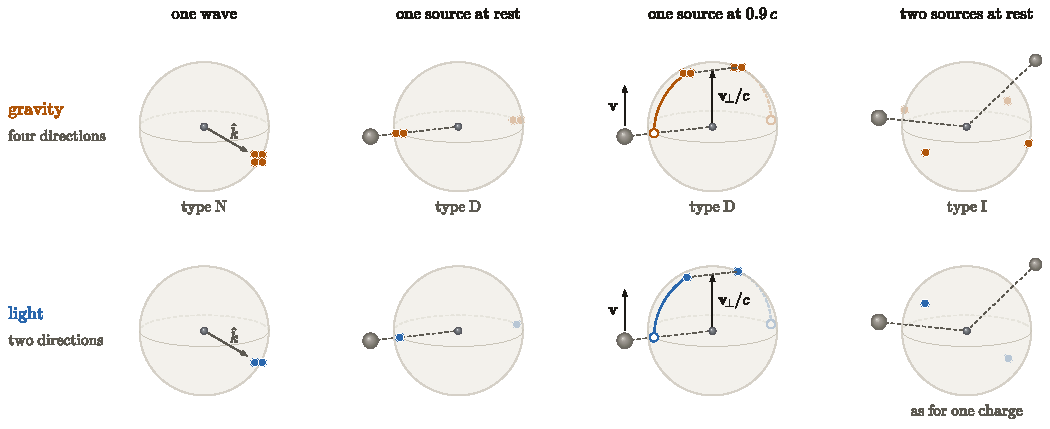
\includegraphics[width=\textwidth]{figures/stars.pdf}
\caption{The stars of a field, the solutions of Eq.~\eqref{eq:stars}, on the
sky around one pixel (each disc), for gravity (top) and light (bottom),
computed in the reference implementation. Coincident stars are drawn as touching
dots, so that every sky of gravity holds four and every sky of light two; faint
dots and dashed lines lie on the far side. One wave puts all of them on its
direction of travel $\hat k$. One source at rest, a mass or a charge, puts them
in two groups on the line through it. Moving across that line at $0.9\,c$, the
source folds both groups toward its velocity, along the paths drawn from their
places at rest (open circles), and the midpoint of the two, as a vector, is its
velocity across the line to where it is now, $\mathbf{v}_\perp/c$,
Eq.~\eqref{eq:star-velocity}. Two masses at rest give four separate stars
(Petrov type I), so they could not be one body; two charges give light's two
stars again, at the ends of the line of force, as one charge would.}\label{fig:stars}
\end{figure*}

\paragraph{Shape.} A plane wave stretches and squeezes only across its
direction of travel, so its tidal tensor has one vanishing eigenvalue and
$\det\tE = 0$. The field of a single mass has eigenvalues in the ratio
$-2 : 1 : 1$, and its determinant is never zero. One reading of one pixel
therefore distinguishes a single wave from a single mass. The test is for an
isolated source: the fields of several masses, or of several waves, add, and
their sum can have either form.

\paragraph{The magnetic part.} In a wave the magnetic tidal tensor is as large
as the electric one; it is the same pattern turned by $45^\circ$ about the
direction of travel. Near slowly moving matter it is smaller by the ratio of
the matter's speed to that of light,
\begin{equation}\label{eq:magnetic-ratio}
\frac{|\tB|}{|\tE|} = 1 \quad\text{(wave)},
\qquad
\frac{|\tB|}{|\tE|} \sim \frac{v}{c} \quad\text{(near field)} ,
\end{equation}
where $|\tE|^2 = \tE_{ij}\tE_{ij}$ (the Frobenius norm) and likewise for $\tB$,
and $v$ is the speed of the matter. At a distance $r$ from a compact source of
size $L$, the part of the field that changes is smaller by about $(v/c)(r/L)$,
that is, by $kr$ at the frequency of the change: more than $v/c$, but still far
below one in the near zone.
Averaged over time, the first holds for any mixture of waves from independent
sources, so the magnetic part is a detector of radiation that the pull of
nearby objects hardly touches. Coherent waves are an exception: in a standing
wave the magnetic part vanishes where the electric part is largest.

\paragraph{Ten numbers: four invariants, three angles, three velocities.} A
reading whose eigenvalues are distinct can be written
\begin{equation}\label{eq:polar}
\mathcal{W} = P\,\mathrm{diag}(w_1, w_2, w_3)\,P^{T}, \qquad
P = R_0\,e^{iK_0},
\end{equation}
with $P$ a complex rotation ($P^TP = 1$), split into a real rotation $R_0$ and an
imaginary one. The three complex eigenvalues, which sum to zero, are four
numbers no observer can change. The rotation $R_0$ gives three angles, the
orientation of the field's own axes. The imaginary part,
$e^{2iK_0} = P^{\dagger}P$, gives three more: the velocity of the one frame in
which $\tE$ and $\tB$ share their axes, the field's own rest frame (the
principal observer of Ref.~\cite{CostaWyllemanNatario2021}; for a field of type I
it is unique, and it is the rest frame of matter only for a stationary
source). Ten numbers, read as four, three and three.

The consequences are immediate. For a scene of masses at rest, $\tB = 0$ in the
scene's frame, so its eigenvalues are real; a pixel moving through it at any
speed still finds real eigenvalues, and finds in $P$ the velocity of the scene
relative to itself. The pixel is a speedometer: it reads its own velocity through
an unknown room, at any speed, with no map of the room. In the reference
implementation, for a pixel moving at $0.6\,c$ past four unknown masses, the
rapidity is recovered to $4\times10^{-8}$. To first order in the speed, in the
principal axes of $\tE$ with eigenvalues $\lambda_a$,
\begin{equation}\label{eq:speedometer}
\tB_{bc} = \frac{v_a}{c}\,(\lambda_c - \lambda_b) \quad ((a,b,c)\ \text{cyclic}),
\qquad \tB_{aa} = 0 ,
\end{equation}
so a pixel whose readings carry white noise $\sigma$ on each component (in the
orthonormal basis of the paragraph \emph{How precisely}) reads
each component of its velocity to within
$c\,\sigma/\sqrt2\,|\lambda_b - \lambda_c|$. A pixel that reads the tide of a
room, $10^{-8}\,\mathrm{s^{-2}}$ near a person, to one part in $10^{8}$, reads its
own speed to about two metres per second.

The converse is an alarm. A pixel moving through a static scene, however fast,
always finds real eigenvalues. If they are complex, something in the scene
moves relative to the rest of it, or turns: the pixel's own motion can never
set it off (Fig.~\ref{fig:speedometer}). The phase of the eigenvalues measures turning. Outside a spinning
body of mass $M$ and angular momentum $J_s = Mca$, the eigenvalues are
proportional to $(r - ia\cos\vartheta)^{-3}$, as in Kerr's solution
\cite{Kerr1963}, so their phase, $3a\cos\vartheta/r$ for $a \ll r$, reads the
spin along the line of sight; for the Earth seen from above a pole it is
$1.5\times10^{-6}$.

\begin{figure}
\centering
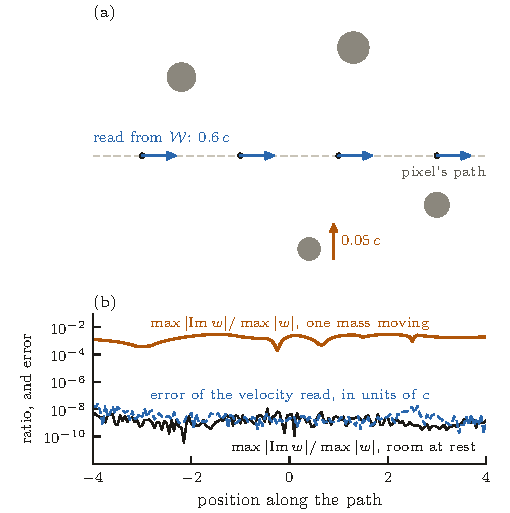
\includegraphics[width=\columnwidth]{figures/speedometer.pdf}
\caption{The speedometer and the alarm. (a) A pixel crosses a room of four
masses unknown to it at $0.6\,c$ (seen from above, in the room's frame), and at
every point reads its own velocity from $\mathcal{W}$ alone, Eq.~\eqref{eq:polar}
(arrows). (b) Along the path: the error of the velocity read (dashed), and the
alarm $\max|\mathrm{Im}\,w|/\max|w|$ over the eigenvalues $w$ of $\mathcal{W}$,
which is zero to rounding for the room at rest, however fast the pixel moves,
and is not when one mass crosses the room at $0.05\,c$. Computed from the exact
field of uniformly moving masses.}\label{fig:speedometer}
\end{figure}

Light cannot do this. Its field at a point has only two invariants,
$\mathbf{E}^2 - c^2\mathbf{B}^2$ and $\mathbf{E}\cdot\mathbf{B}$, and in the frame
where $\mathbf{E}$ is parallel to $\mathbf{B}$ a boost along their common axis
and a turn about it change nothing. A sensor of light is at best a
two-dimensional speedometer. A single body does the same to gravity's field
(type D): coming straight at the pixel, even at $0.3\,c$, it shows no $\tB$ at
all, and its radial speed is unreadable. Two bodies, or one that is not round,
remove the blind spot.

\paragraph{A moving body, exactly.} The four stars of a single body moving at any
speed are its two pairs, displaced by aberration toward its direction of motion.
Their midpoint, as a vector, is exactly its velocity across the line of sight
(Fig.~\ref{fig:stars}):
\begin{equation}\label{eq:star-velocity}
\tfrac12\,(\hat p_+ + \hat p_-) = \frac{\mathbf{v}_\perp}{c} ,
\end{equation}
with $\hat p_\pm$ the directions of the two pairs and $\mathbf{v}_\perp$ the
velocity across the line from the body to the pixel. The reference
implementation finds the two sides equal to $2\times10^{-7}$ at $0.9\,c$. The
ratio $|\tB|/|\tE| = \sqrt3\,v_\perp/c$ of Section~\ref{sec:near-field} is its
first-order form. A body coming straight on shows no sideways velocity and
cannot be ranged (below), but because its tide grows as
$r^{-3}$, the pixel reads when it will arrive,
\begin{equation}\label{eq:contact}
-\frac{r}{\dot r} = \frac{3\,\tE_\parallel}{\dot{\tE}_\parallel},
\qquad
\frac{\tE_\parallel\,\ddot{\tE}_\parallel}{\dot{\tE}_\parallel^2} = \frac43 - \frac{r\ddot r}{3\dot r^2},
\end{equation}
and from the second ratio whether it is coasting ($4/3$), braking or driven.

\paragraph{Separating waves at one point.} Several waves crossing a pixel at
once add their matrices, and the algebra of squares lets one pixel pull them
apart.

At one instant, two waves give $\mathcal{W} = c_1\mathbf{m}_1\mathbf{m}_1^{T} +
c_2\mathbf{m}_2\mathbf{m}_2^{T}$, of rank two, so $\det\mathcal{W} = 0$: two real
conditions that tell two crossing waves from the pull of a mass, whose
$\det\mathcal{W} = -2(GM/r^3)^3$. The vector $\mathbf{v}$ with $\mathcal{W}\mathbf{v} = 0$ is
$\mathbf{m}_1\times\mathbf{m}_2$; the null vectors orthogonal to it are the
roots of one quadratic, and they are $\mathbf{m}_1$ and $\mathbf{m}_2$, which give
both directions and then both amplitudes. This is Sylvester's theorem on sums of
two fourth powers \cite{Sylvester1851} in the language of the sky. Light cannot
do it at all: a single wave already uses four of its six numbers.

At one frequency, three waves can be separated. Writing the reading as
$\mathcal{W}(t) = \mathcal{W}_+e^{-i\omega t} + \mathcal{W}_-e^{i\omega t}$ (since $\mathcal W$ is
complex, $\mathcal W_-$ is not the conjugate of $\mathcal W_+$), both parts are sums
over the same three squares, $\mathcal{W}_\pm = \sum_a \alpha_a^\pm\,
\mathbf{m}_a\mathbf{m}_a^{T}$, and
\begin{equation}\label{eq:pencil}
\det(\mathcal{W}_+ - \lambda\,\mathcal{W}_-) = \det[\mathbf{m}_1,\mathbf{m}_2,\mathbf{m}_3]^2
\prod_{a=1}^{3}(\alpha^+_a - \lambda\,\alpha^-_a) .
\end{equation}
Its three roots give the ratios $\lambda_a = \alpha_a^+/\alpha_a^-$, which must be
distinct (two face-on binaries turning the same way share one; any three distinct
directions give $\det[\mathbf m_1,\mathbf m_2,\mathbf m_3] \neq 0$); at each, one
wave drops out, the null vector of what remains is the cross product of the other
two $\mathbf{m}$, and cross products of those give all three directions. For a
circular binary seen at inclination $\iota$, $|\lambda| = \tan^{\pm4}(\iota/2)$,
so the roots also give the three inclinations. Three binaries in one frequency
bin, which a single interferometer cannot tell apart, are three stars to one
pixel (to $10^{-9}$ in the reference implementation).

Over time, four. If the waves come from fixed directions but carry any
waveforms at all, the readings span a subspace of the five-dimensional space of
matrices; for four waves whose waveforms are linearly independent it is
four-dimensional, and there is one matrix $A$ with
$\mathrm{tr}(A\mathcal{W}) = 0$ for every reading. Each wave's $\mathbf{m}$ then lies on
two conics,
\begin{equation}\label{eq:four-waves}
\mathbf{m}^{T}\!A\,\mathbf{m} = 0, \qquad \mathbf{m}\cdot\mathbf{m} = 0 ,
\end{equation}
and two conics meet in four points: the four directions (Fig.~\ref{fig:voices}).
For light the same argument gives two. In general a point sensor of a field of spin $s$ separates
$s$ plane waves at one instant, $s + 1$ at one frequency and $2s$ from a time
history; for light, $1$, $2$ and $2$, the known limit for electromagnetic vector
sensors \cite{NehoraiPaldi1994,HochwaldNehorai1996}; for gravity, $2$, $3$ and
$4$. In the reference implementation four waves with random waveforms are
located to $10^{-14}$, and to $10^{-4}$ radian with noise of $10^{-4}$ of the
signal on every component over three hundred readings.

\begin{figure*}
\centering
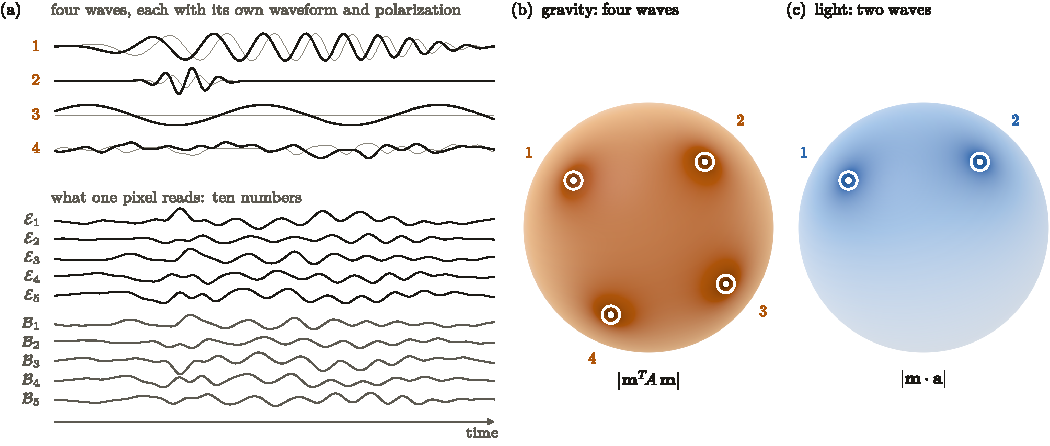
\includegraphics[width=\textwidth]{figures/voices.pdf}
\caption{One pixel, four waves. (a) Four plane waves arrive from four fixed
directions, each with its own waveform in both polarizations (strong and faint lines),
and one pixel reads the ten numbers of $\tE$ and $\tB$ while all four pass.
(b) From the readings alone: the matrix $A$ with $\mathrm{tr}(A\mathcal{W}) = 0$
for every reading, and, on the sky toward the sources, the size of
$\mathbf{m}^{T}\!A\,\mathbf{m}$, shaded over two and a half decades. It vanishes
at exactly four points, Eq.~\eqref{eq:four-waves}: the zeros found from the
readings (dots) fall on the four sources (rings) to $10^{-14}$. (c) Light from
the first two sources, the same way: its readings $\mathbf{E} + ic\mathbf{B}$
span a plane, the vector $\mathbf{a}$ orthogonal to it gives
$\mathbf{m}\cdot\mathbf{a}$, and that vanishes at the two sources; a third wave of
light would fill all six of its numbers and leave nothing to find. Computed in
the reference implementation.}\label{fig:voices}
\end{figure*}

Uncorrelated sources can be separated from second moments alone. In the
frequency domain the two helicities occupy separate halves of the ten numbers,
and the brightness and the circular polarization of the sources give two
five-by-five matrices built from the same five steering vectors; when the
sources' circular fractions differ, diagonalizing one in the frame that whitens
the other separates five sources in closed form, with their directions,
brightnesses and circular fractions (checked in the reference implementation).

\paragraph{What one pixel sees of the sky.} For a sky full of independent
sources overlapping in frequency, what a pixel can learn at each frequency is
its ten-by-ten spectral matrix, one hundred real numbers. Split by helicity, it
holds three blocks: the brightness $I$ and the circular polarization $V$ of the
sky in two five-by-five Hermitian blocks, and the linear polarization in a
complex symmetric one. The brightness enters through the kernel
\begin{equation}\label{eq:pixel-kernel}
\begin{gathered}
\sum_{A=+,\times} e^{A}_{ij}\, e^{A}_{kl}
= P_{ik}P_{jl} + P_{il}P_{jk} - P_{ij}P_{kl},\\
P_{ij} = \delta_{ij} - \hat n_i \hat n_j ,
\end{gathered}
\end{equation}
a polynomial of degree four in the components of $\hat n$, so the pixel sees the
spherical harmonics of $I$ of degree four and below, twenty-five numbers; it
sees as many of $V$, and eighteen of the linear polarization, which carries spin
weight four and enters only at degree four. That is
\begin{equation}\label{eq:sky-count}
25 + 25 + 18 = 68
\end{equation}
numbers of the sky, all independent; the other thirty-two of the hundred vanish
for any sky of gravitational waves and are checks against sensor noise or
anything else. The brightness and the circular polarization never mix at one
pixel: one lives in the real part of the spectral matrix, the other in its
imaginary part. (They mix in the cross-correlation of two separated detectors
\cite{AllenOttewill1997,SetoCooray2004}, through the phase between them.) The
same count for a point sensor of a transverse field of spin $s \ge 1$, with two
helicities, gives $2(2s+1)^2 + 2(4s+1)$: $28$ of $36$ for light. Sound, a
pressure and a velocity, has one longitudinal polarization and is counted
separately: $9$ of $16$. All
three counts are checked in the reference implementation
(Fig.~\ref{fig:sky-count}).

One of the sixty-eight numbers is the handedness of the whole sky. An isotropic
sky of brightness $I$ and net circular polarization $V$ puts exactly
$(V/I)\langle\tE\cdot\tE^*\rangle$ into the imaginary part of
$\langle\tE\cdot\tB^*\rangle$, so one pixel measures
whether the sky is chiral, which a single planar interferometer cannot
\cite{SetoTaruya2007}.

The rest of the sky is invisible to second moments. The twelve corners of a
regular icosahedron form a spherical design of degree five: they average every
polynomial of degree five or less exactly as the whole sphere does
\cite{Delsarte1977}. Twelve equal, unpolarized, independent sources at those
corners therefore give a pixel exactly the second moments of a uniform sky,
while six at the corners of an octahedron, a design of degree three only, do
not; the reference implementation finds the first pair equal to one part in
$10^{15}$. Sources that are not Gaussian say more: the fourth moments of the
pixel are kernels of degree eight, which no icosahedron averages. Two pixels a
wavelength apart tell the two skies apart as well, because their
cross-correlation carries the phase $e^{i\omega\hat n\cdot\Delta\mathbf x/c}$,
which no finite design averages exactly.

\begin{figure*}
\centering
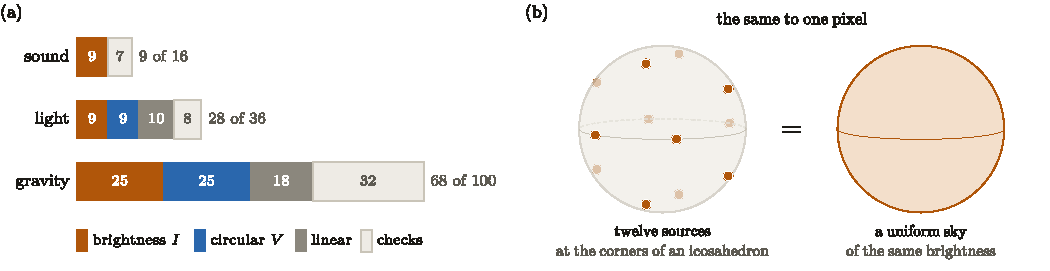
\includegraphics[width=\textwidth]{figures/sky-count.pdf}
\caption{What one pixel sees of the sky at one frequency. (a) Of the real
numbers in the spectral matrix of a point sensor, those that carry the sky's
brightness $I$, its circular polarization $V$ and its linear polarization, and
those that vanish for any sky of waves and serve as checks,
Eq.~\eqref{eq:sky-count}, for sound (a pressure and a velocity), light and
gravity. (b) What a pixel cannot see: twelve equal, unpolarized, independent
sources at the corners of a regular icosahedron give it exactly the second
moments of a uniform sky of the same total brightness, because those corners
average every polynomial of degree five or less as the whole sphere
does.}\label{fig:sky-count}
\end{figure*}

\paragraph{How far away is a wave source?} A single plane wave has no distance.
The field of a real source at distance $r$ is not quite a plane wave: it carries
terms falling as $1/r^2$, $1/r^3$ and beyond, organized by how they turn about
the line of sight \cite{Sachs1962}, and a pixel sees them. At one instant the
departure of the oscillating part of $\mathcal{W}$ from rank one, the ratio of its
second singular value to its first (the singular values $s_1 \ge s_2 \ge s_3$
being the square roots of the eigenvalues of $\mathcal W^\dagger\mathcal W$, not
the eigenvalues of $\mathcal W$, which all vanish for a wave), is
\begin{equation}\label{eq:ranging-instant}
\frac{s_2}{s_1} = \frac{C(\iota, \theta)}{(kr)^2} + O\bigl((kr)^{-3}\bigr),
\end{equation}
not $1/kr$: the first correction, $\mathbf m\,\delta\mathbf m^T + \delta\mathbf m\,\mathbf m^T$
with $\delta\mathbf m \propto \hat k$, equals $(\mathbf m + \delta\mathbf m)(\mathbf m +
\delta\mathbf m)^T$ to that order, and only tilts the apparent $\mathbf{m}$, which at one
instant cannot be told from a tilt of the source. The oscillating part is read
at one instant from $\dot{\mathcal W}$, which holds none of the static tide of the
pair's mass, $(c/v)^2$ times larger than the departure. For two masses turning in a
circle, seen at inclination $\iota$ and wave phase $\theta$,
\begin{equation}\label{eq:ranging-C}
\begin{gathered}
C = \frac{2\sin^2\!\iota\,\sqrt{A^2 + B^2}}{D}, \qquad
B = 2\cos\iota\,\sin\theta\cos\theta,\\
A = (1 - 3\cos^2\!\iota)\cos^2\!\theta - 4\cos^2\!\iota\,\sin^2\!\theta,\\
D = (1 + \cos^2\!\iota)^2\cos^2\!\theta + 4\cos^2\!\iota\,\sin^2\!\theta,
\end{gathered}
\end{equation}
which is $2$ for any phase seen edge on and, at the phases $\theta = 0$ and
$\pi$, vanishes at the angle $\cos^2\iota = 1/3$. Over a cycle more can be done. The two frequency parts
$\mathcal{W}_\pm$ (the parts at $e^{\mp i\omega t}$, whose amplitudes go as
$\cos^4(\iota/2)$ and $\sin^4(\iota/2)$) depart from rank one by
$2\tan^{\pm2}(\iota/2)/(kr)^2$, both with the same $s_2$, so that
$kr = [2\sqrt{s_1(\mathcal{W}_+)s_1(\mathcal{W}_-)}/s_2(\mathcal{W}_+)]^{1/2}$ needs no knowledge of the
inclination. And the first-order tilt, invisible at one instant, differs between
the two helicities: the directions read from the two parts differ by
\begin{equation}\label{eq:helicity-split}
\Delta\theta_\pm = \frac{8\,|\cot\iota|}{kr} .
\end{equation}
Equation~\eqref{eq:helicity-split} holds while $\tan^2(\iota/2)$ and
$\cot^2(\iota/2)$ both exceed $1/kr$; near face-on the weaker helicity's
amplitude falls as $\tan^4(\iota/2)$, so its direction, not the formula, limits
the range, and a full fit over distance, inclination and orientation gives the
best inclination. A difference of directions measured at signal-to-noise ratio $\rho$ ranges the
source out to $kr$ of order $\rho$, where the rank departure reaches only $kr$
of order $\sqrt\rho$. A source seen at $\rho = 10^{3}$ can be ranged out to
several hundred reduced wavelengths: at $100\,\mathrm{Hz}$, a few hundred
thousand kilometres. The
reference implementation checks Eqs.~\eqref{eq:ranging-C}
and~\eqref{eq:helicity-split} against the exact field of a turning pair to
within a few per cent at $kr = 80$ and $0.5$ per cent at $kr = 200$
(Fig.~\ref{fig:ranging}).

\begin{figure*}
\centering
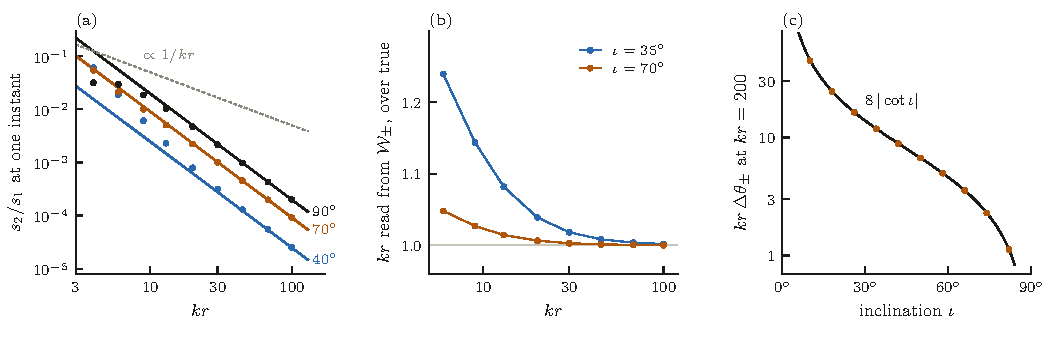
\includegraphics[width=\textwidth]{figures/ranging.pdf}
\caption{Ranging a wave source from one pixel: the exact field of two equal
masses turning in a circle, read at reduced distance $kr$ and inclination
$\iota$ (points), against the formulas (lines). (a) At one instant, at wave
phase $\theta = 0$, the oscillating part of $\mathcal{W}$ departs from rank one
by $C(\iota, 0)/(kr)^2$, Eqs.~\eqref{eq:ranging-instant}
and~\eqref{eq:ranging-C}, not by $1/kr$ (dashed); the points approach the lines
as the next order dies away. (b) Over a cycle, the distance read from the two
frequency parts $\mathcal{W}_\pm$ alone, with no knowledge of the inclination,
over the true distance. (c) The directions read from the two frequency parts
differ by $8|\cot\iota|/kr$, Eq.~\eqref{eq:helicity-split}, here at
$kr = 200$.}\label{fig:ranging}
\end{figure*}

\paragraph{The camera sees the present.} The field of a body moving uniformly is
its static field carried along, so it depends on where the body is now. The
stretch axis of $\tE$ points at the body's present position, at any speed (to
$10^{-7}$ radian at $0.3\,c$ in the reference implementation), while its light
shows its position a light-travel time ago, displaced by the aberration angle,
about $v_\perp/c$ (Fig.~\ref{fig:present}). Near two masses in orbit the changing part of the field is
Newton's field of their present positions to order $(kr)^2$, while their
retarded positions would be off by $kr$ itself: at $kr = 0.1$, a tenth of a per
cent against ten per cent. The first-order retardation cancels because mass and
momentum are conserved. The gravitational Sun is therefore $20.5''$ ahead of the
optical Sun along its yearly path across the sky. Laplace took the absence of
gravitational aberration to mean that gravity is far faster than light; it is
what general relativity predicts \cite{Carlip2000}. A camera that sees mass sees
it on its own slice of simultaneity. When a body changes its motion, the field
goes on pointing at where it would have been until the news, travelling at the
speed of light as a wave, arrives.

\begin{figure}
\centering
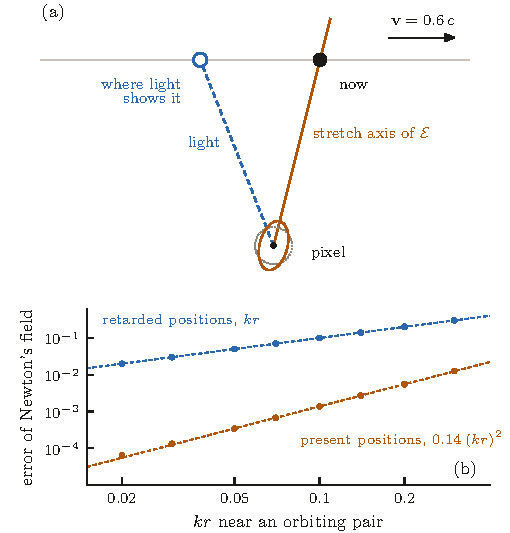
\includegraphics[width=\columnwidth]{figures/present.pdf}
\caption{The camera sees the present. (a) A mass passing a pixel at $0.6\,c$:
the stretch axis of its exact field at the pixel (a ring of free masses,
exaggerated) points at where the mass is now, while its light arrives from where
it was a light-travel time ago. (b) Near two masses in orbit, at reduced
distance $kr$, the changing part of the exact field against Newton's field of
the masses at their present positions, which it matches to order $(kr)^2$, and
at their retarded positions, which miss by $kr$. Computed in the reference
implementation.}\label{fig:present}
\end{figure}

\paragraph{Beyond general relativity, in one reading.} Other theories of gravity
allow up to six polarizations, and waves that travel at other speeds
\cite{EardleyLeeLightman1973}. For any plane wave of the metric, of any
polarization and phase speed $v_p$, the second Bianchi identity gives, with no
field equations assumed,
\begin{equation}\label{eq:bianchi-wave}
\tB_{ij} = \frac{c}{v_p}\,\epsilon_{ipq}\hat k_p\,\tE_{qj} .
\end{equation}
So one reading of $\tE$ (now with a trace, six numbers) and $\tB$ (with an
antisymmetric part, eight) gives the direction, the phase speed, all six
polarizations, and five checks that they belong to one wave. Summing
$\mathbf e_j \times \mathbf b_j$ over the columns of $\tE$ and $\tB$ turns
Eq.~\eqref{eq:bianchi-wave} into a linear equation for
$\mathbf p = (c/v_p)\hat k$,
\begin{equation}\label{eq:wave-vector}
\bigl(|\tE|^2 - \tE^2\bigr)\,\mathbf p = \textstyle\sum_j \mathbf e_j\times\mathbf b_j ,
\end{equation}
whose matrix is invertible whenever $\tE$ has rank two or more; the residual
$\tB - [\mathbf p]_\times\tE$ then tests that the reading is one wave. A purely longitudinal wave, $\tE \propto \hat k\hat k$,
has $\tB = 0$, and its speed cannot be read at one point. In general relativity $v_p = c$ and only the two tensor
polarizations appear. A massive graviton and a massive scalar differ even in
sign: with $n = c/v_p$, the helicity-zero wave of a Fierz--Pauli graviton
\cite{FierzPauli1939} has longitudinal and breathing amplitudes in the ratio
$-2(1 - n^2)$, a scalar wave $+(1 - n^2)$ (Fig.~\ref{fig:beyond}). These are
checked against curvature computed from the metric in the reference
implementation. Testing general
relativity this way at the level of present bounds would need extraordinary
signal-to-noise ratios; what is new is that it needs only one point.

\begin{figure*}
\centering
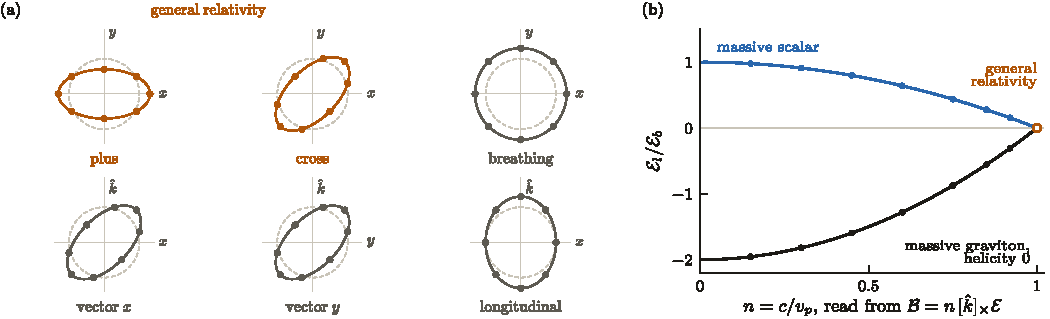
\includegraphics[width=\textwidth]{figures/beyond.pdf}
\caption{Beyond general relativity in one reading. (a) The six polarizations a
metric theory of gravity allows \cite{EardleyLeeLightman1973}, each drawn as the
distortion it makes of a ring of free particles in the plane where it acts
(dashed: at rest; exaggerated), for a wave travelling along $\hat k$; general
relativity has only the first two. One reading gives all six, with the
direction and the phase speed, Eq.~\eqref{eq:bianchi-wave}. (b) The ratio of the
longitudinal to the breathing amplitude, and $n = c/v_p$, both read from one
reading, for the helicity-zero wave of a massive graviton and for a massive
scalar (points: curvature computed from the metric), against $-2(1 - n^2)$ and
$+(1 - n^2)$ (lines). The two differ in sign at every speed, and both ratios
vanish as the speed approaches $c$.}\label{fig:beyond}
\end{figure*}

\paragraph{Matter at the pixel.} Inside matter the pixel reads the density
locally, whatever the matter is: in full,
$\mathrm{tr}\,\tE = 4\pi G[\rho + (p_1 + p_2 + p_3)/c^2]$, with $p_a$ the
principal stresses (so $3p$ for a fluid), less $2\Omega^2$ if the pixel's frame
turns at $\Omega$. The dark matter around the Sun, $0.4\,\mathrm{GeV\,cm^{-3}}$,
gives $6\times10^{-31}\,\mathrm{s^{-2}}$, by its mass alone and with no other
interaction. Between two plates a micrometre apart the Casimir energy density $u$ is
negative; the stress across the plates is $3u$ and the two along them $-u$
each, since the field has no trace, so the sum of stresses is $u$ and the trace,
$8\pi Gu/c^2$, is $-8\times10^{-30}\,\mathrm{s^{-2}}$. The cosmological constant gives
$-\Lambda c^2 = -1\times10^{-35}\,\mathrm{s^{-2}}$. Where radiation streams
through with energy flux $\mathbf F$, as neutrinos from a supernova do, the trace
is $8\pi G|\mathbf F|/c^3$ and the antisymmetric part of $\tB$,
$-(4\pi G/c^3)\,\epsilon_{ijk}F_k$, gives the flux as a vector
(Section~\ref{sec:pixel}), so that
one reading inside the passing shell points back to the star, even when the
collapse is perfectly spherical and sends out no waves at all.

\paragraph{One pixel and many.} A single pixel already does part of a camera's
work, as the paragraphs above show: it places one wave by Eq.~\eqref{eq:one-wave},
separates up to four from their time history, and sees the sky's brightness in
its patterns of degree four and below. An array adds to this in two ways. Its
size sharpens the image, Eq.~\eqref{eq:diffraction}. And it multiplies the
number of sources that can be told apart: an array of $N$ pixels, wherever they
are placed and even along one line, has $5N$ independent steering vectors at
each frequency and helicity, so subspace methods separate up to $5N - 1$
uncorrelated sources, against $N - 1$ for scalar sensors and $3N - 1$ for sensors
of light. The tensor nature of each pixel also removes the false images of a
sparse array. Two scalar sensors far apart see a source equally well at any of
the fringes of their pattern; two pixels $D$ apart see the fringe at the
source's true direction more strongly than its neighbours, because their
response to two directions an angle $\vartheta$ apart is multiplied by
$\cos^8(\vartheta/2)$. With a minimum-variance (Capon) estimator and a source
at signal-to-noise ratio $\rho$, the true fringe stands above the nearest false
one by the factor $1 + \rho^2[1 - \cos^8(\vartheta_1/2)]$, where
$\vartheta_1 \approx \lambda/D$ is the fringe spacing, so that two pixels a
hundred wavelengths apart form a telescope without ambiguity once $\rho$ exceeds
about a hundred (Fig.~\ref{fig:two-pixels}). The reference implementation checks
these three statements.

\begin{figure}
\centering
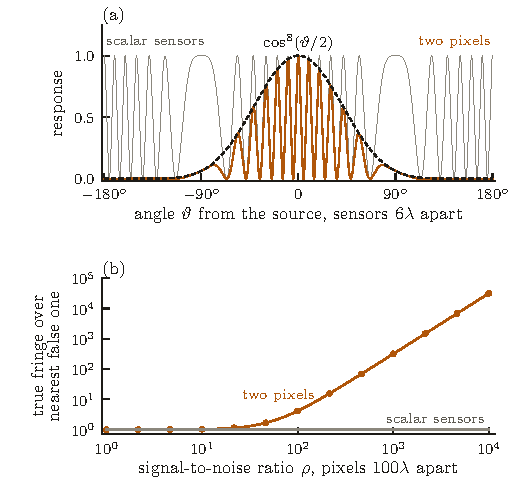
\includegraphics[width=\columnwidth]{figures/two-pixels.pdf}
\caption{Two pixels far apart. (a) The response of two sensors six wavelengths
apart to one source, against the angle from it in the plane of their baseline:
scalar sensors answer equally at every fringe, while for two pixels each fringe
is weighed by $\cos^8(\vartheta/2)$, the overlap of their tensor responses to
the two directions. (b) With a minimum-variance (Capon) estimator and two pixels
a hundred wavelengths apart, the true fringe over the nearest false one,
$1 + \rho^2[1 - \cos^8(\vartheta_1/2)]$ (line; points computed), against the
signal-to-noise ratio; for scalar sensors the two are equal at any
$\rho$.}\label{fig:two-pixels}
\end{figure}

\paragraph{Variation across the array.} A wave of wavelength $\lambda$ changes
across an array of width $a$ by a fraction of order $2\pi a/\lambda$. The field
of a mass at distance $r$, which falls as $1/r^{3}$, changes by a fraction of
order $3a/r$. For a one-metre array, a wave at $100\,\mathrm{Hz}$ and a person
three metres away, these are $2\times10^{-6}$ and $1$. Subtracting the
average over the array therefore removes the wave and keeps the variation of
the neighbourhood. The reverse is harder: the average itself contains the pull
of everything nearby, and the person alone adds $3\times10^{-10}\,\mathrm{s^{-2}}$
to it, a million times the tidal field of the waves LIGO detects. To isolate
the wave the camera must model the nearby masses from their variation and
subtract them, which is how observatories plan to remove the changing pull of
their surroundings \cite{Harms2019,Chaibi2016}, or use the magnetic part, or
compare two arrays far apart; a camera simply keeps what the observatories
throw away. With two arrays far apart the separation is cleaner still: a wave
appears in both, with a delay that gives its direction, while a nearby mass
appears in one. The accompanying demonstrations show the tidal tensor itself
on a slice through the scene, coloured by the direction of stretching in the
manner of diffusion tensor imaging.

\paragraph{Depth.} The same variation measures distance. For an isolated mass
the tidal field goes as $M/r^{3}$ and its gradient as $M/r^{4}$, so their
ratio gives $r$, and then $M$: a pixel and its neighbours locate and weigh a
body with no need to move the camera. This is the principle by which a
calibration rotor's distance from a detector's mirror is found from the ratio
of two of its multipoles \cite{Inoue2018}. A single pixel can range a moving
mass without neighbours, but only with its magnetic part. The electric record
alone cannot do it: the record of a mass $M$ moving along $\mathbf{x}(t)$ is
unchanged if the path is enlarged $\lambda$-fold and the mass
$\lambda^3$-fold, while $\tB$ grows $\lambda$-fold, because the speed of light
supplies the scale. From Eq.~\eqref{eq:magnetic-point}, $\tB\hat n =
(3GM/cr^3)\,\hat n\times\mathbf v$ and $P\dot{\tE}\hat n = -(3GM/r^4)\,\mathbf
v_\perp$, with $P = 1 - \hat n\hat n$, so that
\begin{equation}\label{eq:one-pixel-range}
\hat n\times(\tB\hat n) = \frac{r}{c}\,P\dot{\tE}\hat n ,
\qquad r = c\,\frac{|\tB\hat n|}{|P\dot{\tE}\hat n|} ,
\end{equation}
and then $M$ from $\tE$. The stretch axis of $\tE$ gives $\hat n$ only up to
sign; reversing it leaves the left side of the vector relation unchanged and
reverses the right, so the sign that makes $r$ positive fixes $\hat n$. The reference implementation recovers distance, mass and velocity
this way from the finite-difference curvature of a moving mass. Motion straight
toward or away from the pixel gives no range, though it gives the time of
arrival, Eq.~\eqref{eq:contact}; and the magnetic signal, smaller by $v/c$, sets
the noise. For waves, range comes from the curvature of the wavefront, which
across an array of width $D$ amounts to a phase of order one at the distance
$D^{2}/\lambda$; beyond it range is still measured, with a fractional error of
order $\lambda r/\mathcal{R}D^{2}$ at signal-to-noise ratio $\mathcal{R}$. A
single pixel also ranges a wave source, from how its field departs from that of
a plane wave, Eq.~\eqref{eq:helicity-split}.

\paragraph{Front and back.} A flat array that records only the normal
component $\tE_{zz}$ cannot tell a mass in front of it from the mirror image of
that mass behind it, because the two give the same $\tE_{zz}$ on the plane. The
shear components $\tE_{xz}$ and $\tE_{yz}$ change sign between the two, so the
full tensor separates the half-spaces: a camera with no housing to block
gravity can still ignore the photographer standing behind it.

\paragraph{Three dimensions.} The pixels need not lie in a plane. A closed
shell of pixels sees the whole sky at once and has no blind side; pixels
filling a volume sample the field itself, although, as long as they stay
outside the matter, the ambiguity of Section~\ref{sec:near-field} remains. And in the thermal regime the transparency of matter makes a
further thing possible. Each image is then a set of line integrals, exactly
the data of a medical tomograph. Images from several positions can be combined
into a true three-dimensional map of emissivity, with nothing hidden behind
anything else.

\paragraph{How precisely.} With white noise $\sigma$ on each of the ten numbers,
taken as the coefficients of $\tE$ and $\tB$ in an orthonormal basis of
symmetric trace-free tensors ($e^A_{ij}e^B_{ij} = \delta^{AB}$, so that an
off-diagonal entry carries $\sigma/\sqrt2$), and $\rho = |\mathcal{W}|/\sigma$, one pixel places one wave to within $1/\rho$ radian in
each direction, against $\sqrt2/\rho$ for a sensor of light at the same
signal-to-noise ratio; it reads its own velocity as given after
Eq.~\eqref{eq:speedometer}; and it ranges a moving mass with the precision of
Eq.~\eqref{eq:magnetic-range} below. Table~\ref{tab:one-pixel} sets these
counts beside those of a sensor of light.

How well each of these works against noise follows from the Cram\'er--Rao
bounds of the same fields, which the reference implementation computes and
checks against fits to simulated noisy readings (Fig.~\ref{fig:separation-noise});
the details are collected in Appendix~\ref{app:benchmarks}.

\paragraph{Separation with noise.} Take a wave at $100\,\mathrm{Hz}$ of strain
$10^{-21}$ and, $3\,\mathrm{m}$ from the camera, a rotor of two
$1\,\mathrm{kg}$ masses $12\,\mathrm{cm}$ apart turning 50 times a second,
about the quadrupole of the rotor that calibrates LIGO by its pull
\cite{Ross2021}. Its changing tide has the wave's frequency and a hundred times
its size. Shape alone tells an isolated wave from an isolated mass: the nearest
wave to the field of a mass, and the nearest mass to a wave, lie at half the
reading's size, so one reading of $\tE$ puts the two $\rho/2$ standard
deviations apart, and at $\rho = 12$ fewer than one reading in a hundred is
taken for the other. A wave and a near field together are separated by the
magnetic part, at a fixed price. Let the near field's $\tE$ at the wave's
frequency be anything at all, and its $\tB$ below the noise. Fitting both then
enlarges the error of the wave's amplitude by exactly $\sqrt2$, however strong
the near field: the near field takes the wave's $\tE$, and the wave is read from
its $\tB$, which carries half its signal. Ignored, the rotor would be read as a
wave 35 times the true one; its own magnetic part, smaller than its $\tE$ by
about $kr$ (Eq.~\eqref{eq:magnetic-ratio}), leaks less than $10^{-4}$ of the
wave. An array that reads only $\tE$ must instead model the rotor from its
variation, and pays more: the factor on the wave's error grows as $r/b$ for
neighbours at distance $b$, because a quadrupole's tide falls as $r^{-5}$, and
is $2.2$ for the rotor and an array a metre across, or $1.26$ with $\tB$ as well.

\paragraph{How well depth is measured.} For one mass the field and its gradient
give the range exactly, $r = \sqrt{15}\,|\tE|/|\nabla\tE|$ with norms over all
components, and the Cram\'er--Rao bounds on range and mass are
\begin{equation}\label{eq:depth-bound}
\Bigl(\frac{\sigma_r}{r}\Bigr)^2 = \frac{1}{\rho_E^2} + \frac{1}{\rho_G^2},
\qquad
\Bigl(\frac{\sigma_M}{M}\Bigr)^2 = \frac{16}{\rho_E^2} + \frac{9}{\rho_G^2},
\end{equation}
where $\rho_E$ and $\rho_G$ are the signal-to-noise ratios of the field and of
its gradient, whatever the direction. A pixel with six neighbours at distance
$b \ll r$ has $\rho_E = \sqrt7\,\rho$ and $\rho_G = \sqrt{30}\,\rho\,b/r$, so
$\sigma_r/r \approx r/(\sqrt{30}\,\rho b)$. This rests on Euler's relation for a
field homogeneous of degree $-N$ about its source, $(\mathbf{x}_s -
\mathbf{x})\cdot\nabla f = N f$, with $N = 3$ for the tide of a mass, by which
geophysicists find the depth of buried sources from measured gradients
\cite{Thompson1982,Reid1990}. The magnetic part of one pixel,
Eq.~\eqref{eq:one-pixel-range}, ranges a moving mass with no neighbours to
\begin{equation}\label{eq:magnetic-range}
\frac{\sigma_r}{r} = \frac{1}{\rho_B} ,
\end{equation}
$\rho_B$ the signal-to-noise ratio of $\tB$ alone, $\sqrt3\,v_\perp/c$ times
that of $\tE$ in each reading: for a person walking at
$1.4\,\mathrm{m\,s^{-1}}$, a hundred million times worse than with neighbours.
Depth along one line is the limit. For bodies on one line through the pixel
every derivative of $\tE$ there has the pattern of a single mass, so field and
gradient see one body at $r_{\mathrm{eff}} = \sum_i M_i r_i^{-3} / \sum_i M_i
r_i^{-4}$, weighted toward the nearer: two equal masses $\Delta$ apart appear
as one at $r - \Delta^2/r$, and a rod pointing at the camera as a point nearer
than its centre. The spread of the depths shows first in the second
derivatives, so two equal masses on one line are told from one only when
$\Delta$ exceeds about $0.7\,(r^2/b)/\rho^{1/2}$: the square-root law that
Section~\ref{sec:near-field} found for masses side by side. A round body of any
size is a point, and its size is not measured at all.

\begin{figure*}
\centering
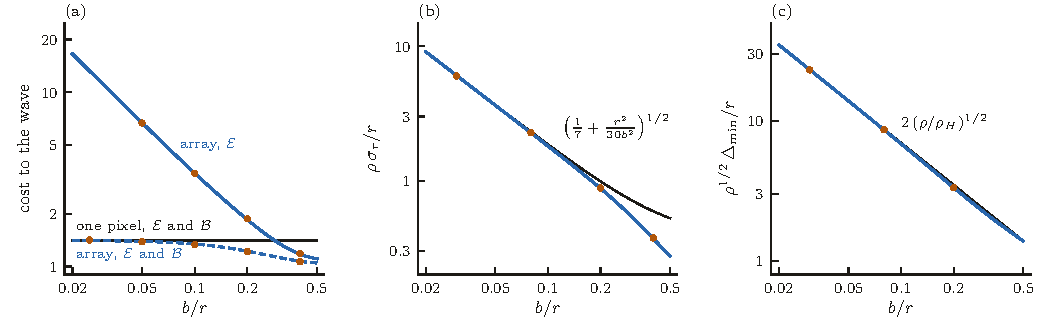
\includegraphics[width=\textwidth]{figures/separation-noise.pdf}
\caption{Separation and depth with noise, against the distance $b$ of a pixel's
six neighbours over the distance $r$ of the source. Blue: Cram\'er--Rao bounds
of the full models; black: closed forms; dots: the spread of
maximum-likelihood fits to simulated noisy readings. (a) The factor $D$ by
which fitting the rotor of the text enlarges the error of a wave's amplitude:
at one pixel from $\tE$ and $\tB$, with any near field, $\sqrt2$ (the dot at
left is a simulation with the rotor present); for the array, which fits the
rotor as a point quadrupole of unknown moment and position, from $\tE$ alone
(solid) and from both (dashed). (b) The range of one mass, with $\rho$ the
signal-to-noise ratio of one pixel's reading, against
Eq.~\eqref{eq:depth-bound}. (c) The separation $\Delta_{\min}$ in depth at which
two equal masses on one line are told from one at one standard deviation.
Computed in the reference implementation.}\label{fig:separation-noise}
\end{figure*}

\begin{table}
\centering
\begin{tabular}{p{0.46\linewidth}p{0.12\linewidth}p{0.13\linewidth}p{0.14\linewidth}}
At one point & Sound & Light & Gravity \\ \hline
Numbers recorded & 4 & 6 & 10 \\
Numbers no observer can change & -- & 2 & 4 \\
Own velocity readable, components & -- & 2 & 3 \\
Waves separated at one instant & 1 & 1 & 2 \\
Waves separated at one frequency & -- & 2 & 3 \\
Waves separated over time & 2 & 2 & 4 \\
Sky numbers per frequency (of) & 9 (16) & 28 (36) & 68 (100) \\
Direction of one wave, standard deviation & -- & $\sqrt2/\rho$ & $1/\rho$ \\
\end{tabular}
\caption{What a sensor at one point can know, for sound (pressure and velocity),
light (electric and magnetic fields) and gravity (the ten numbers of a pixel).
Separation counts are for plane waves from distinct directions; over time the
waveforms are arbitrary. A dash marks an entry that does not
apply.}\label{tab:one-pixel}
\end{table}